\documentclass[12pt, letterpaper]{article}
\usepackage[spanish]{babel}
\usepackage[utf8]{inputenc}
\usepackage{graphicx}
\usepackage{amssymb}
\graphicspath{{./imagenes/}}
\usepackage{xcolor}

%Paquetes para símbolos y entornos matematicos. En este documento se usa para poder usar el tag \begin{align} y \begin{align*} que permiten alinear expresiones matemáticas
\usepackage{amsmath}
\usepackage{amssymb}
%paquete que permite el uso de del argumento H al momento de insertar imágenes
\usepackage{float}

%comando para especificar el título del documento 
\title{Matemáticas para las Ciencias Aplicadas I}

%comando para especificar el autor del documento
\author{Pérez Romero Natalia Abigail}

%comando para especificar la fecha del documento
\date{\today}
%--------------Fin preámbulo--------------

%------------Inicio documento-------------
\begin{document}
%comando que genera el titulo con los datos especificados en el preámbulo
\maketitle
\textbf{Tarea XIV. Ejercicios del libro Cálculo. Una variable de Thomas J.R, George B.}

\textbf{Ejercicios 2, 28, 31 y 32 de  la sección 2.7 Tangentes y Derivadas}

\textbf{2.  } Use cuadrícula y una regla para estimar de manera general la pendiente de la curva (en unidades de y por unidades de x) en los puntos P1 y P2. \\

\begin{figure}[tbh]
\centering
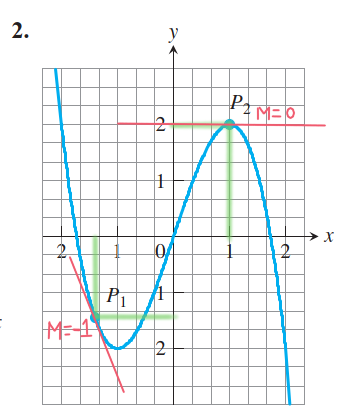
\includegraphics[width=20em]{t14uno}
\end{figure}


\textbf{28. Velocidad de un cohete} A $t$ segundos del despegue, la altura de un cohete es de $3t^2$ pies. ¿Cuál es la velocidad de ascenso del cohete 10 segundos después del lanzamiento?

$$V(t) = \lim_{ h \to 0} \frac{3(10+h)^2 - 3(10)^2}{h} =   \lim_{ h \to 0} \frac{3(100+20h+h^2) - 3(100)}{h} = $$
$$\lim_{ h \to 0} \frac{300+60h+6h^2 - 300}{h} = \lim_{ h \to 0} \frac{60h+6h^2}{h}= \lim_{ h \to 0} \frac{h(60 + 6h)}{h} $$
$$\lim_{ h \to 0} (60 + 6h) = 60 \text{ pies/segundos}$$

\textbf{31.}¿La gráfica de

\begin{align*}
f(x)= \left\{ \begin{array}{lcc}
                 x^2 \sen (1/x), &   si   & x \neq 0 \\
             	\\ 0, &   si   & x = 0
             \end{array}
   \right.
\end{align*}
tiene una tangente en el origen? Justifique se respuesta.

Sí, preguntar si tiene una tangente en el origen es lo mismo que preguntar si es derivable en el origen si es derivable en el origen entonces el límite existe cuando $x \to 0$.\\

$$f'(x) =\lim_{ h \to 0} \frac{( h^2 \sen 1/h - f(0))}{h} = \lim_{ h \to 0} \frac{h^2 (\sen 1/h)}{h} = \lim_{ h \to 0} h \sen 1/h $$

El límite existe por lo tanto es derivable por lo tanto tiene una tangente en el origen.

\begin{figure}[tbh]
\centering
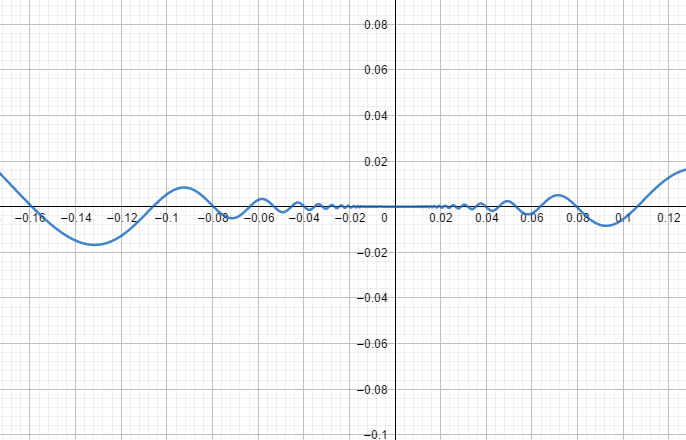
\includegraphics[width=30em]{t14dos}
\end{figure}
\newpage

\textbf{32.}¿La gráfica de

\begin{align*}
g(x)= \left\{ \begin{array}{lcc}
                 x \sen (1/x), &   si   & x \neq 0 \\
             	\\ 0, &   si   & x = 0
             \end{array}
   \right.
\end{align*}
tiene una tangente en el origen? Justifique se respuesta.

No,

$$g'(x) =\lim_{ h \to 0} \frac{( h \sen 1/h - f(0))}{h} = \lim_{ h \to 0} \frac{h (\sen 1/h)}{h} = \lim_{ h \to 0}  \sen 1/h $$

El límite no existe por lo tanto es no derivable por lo tanto no tiene una tangente en el origen.

\end{document} 